%%% Uncomment the following for normal slide show
\documentclass[10pt,serif,professionalfont]{beamer}

%%% or uncomment this for handouts
% \documentclass[handout,ignorenonframetext]{beamer}

%%% or uncomment this for the article version
% \documentclass[11pt]{article}
% \usepackage{beamerarticle}

%%% Based on a TeXnicCenter-Template by Tino Weinkauf.
%%%%%%%%%%%%%%%%%%%%%%%%%%%%%%%%%%%%%%%%%%%%%%%%%%%%%%%%%%%%%

%\usepackage[utf8]{inputenc}
\usepackage[ansinew]{inputenc}

\usepackage[english]{babel}
%\usepackage[bibnewpage]{apacite}
%\usepackage{natbib}

\usepackage{fancyhdr}
\usepackage{setspace}
\usepackage{indentfirst}
\usepackage{booktabs}

\usepackage{amsmath, amsbsy, amssymb}

\usepackage{graphics}
\usepackage{graphicx}
\usepackage{subfig}
\usepackage{caption}
\usepackage{float}
\usepackage{rotating}
\usepackage{pdflscape}
\usepackage{caption}

\usepackage{soul} %for highlighting for mark?
\usepackage{color}
%\sethlcolor{white}




%%%%%%%%%%%%%%%%%%%%%%%%%%%%
%%% Beamer Stuff
%%%%%%%%%%%%%%%%%%%%%%%%%%%%

\let\Tiny=\tiny

\mode<article>
{
  \usepackage{fullpage}
  \usepackage{pgf}
  \usepackage{hyperref}
  \setjobnamebeamerversion{example.beamer}
}

\mode<presentation>
{
  % \usetheme{Dresden}
  % \usetheme{Marburg}
  % \usetheme{Hannover}
  \usetheme{Singapore}
  % \useoutertheme{smoothbars}
  % \useoutertheme{infolines}
  \usecolortheme{seagull}
  \setbeamercovered{invisible}
  \setbeamertemplate{navigation symbols}{}%remove navigation symbols
%  \setbeamertemplate{footline}[page number]
  \setbeamertemplate{footline}[frame number]
}

\mode<handout>
{
%%% In handout mode give the individual pages a light grey background
\setbeamercolor{background canvas}{bg=black!5}
%%% Put more than one frame on each page to save paper.
\usepackage{pgfpages}
\pgfpagesuselayout{4 on 1}[letterpaper,border shrink=3mm, landscape]
% \pgfpagesuselayout{2 on 1}[letterpaper,border shrink=5mm, portrait]
% \setbeameroption{show notes}
}
% \usepackage[latin1]{inputenc}

\setbeamertemplate{itemize items}[default]
\setbeamertemplate{enumerate items}[default]
\setbeamertemplate{frametitle continuation}[from second]

\setbeamercovered{transparent}

%\usepackage{appendixnumberbeamer}

\usepackage[T1]{fontenc}
\usepackage[osf]{mathpazo}
%\linespread{1.05}         % Palatino needs more leading (space between lines)

%\usepackage{pxfonts}
%\usepackage{eulervm}

 %David I didn't have access to this file!!!
%% Based on a TeXnicCenter-Template by Tino Weinkauf.
%%%%%%%%%%%%%%%%%%%%%%%%%%%%%%%%%%%%%%%%%%%%%%%%%%%%%%%%%%%%%

%\usepackage[utf8]{inputenc}
\usepackage[ansinew]{inputenc}

\usepackage[english]{babel}
%\usepackage[bibnewpage]{apacite}
%\usepackage{natbib}

\usepackage{fancyhdr}
\usepackage{setspace}
\usepackage{indentfirst}
\usepackage{booktabs}

\usepackage{amsmath, amsbsy, amssymb}

\usepackage{graphics}
\usepackage{graphicx}
\usepackage{subfig}
\usepackage{caption}
\usepackage{float}
\usepackage{rotating}
\usepackage{pdflscape}
\usepackage{caption}

\usepackage{soul} %for highlighting for mark?
\usepackage{color}
%\sethlcolor{white}




%%%%%%%%%%%%%%%%%%%%%%%%%%%%
%%% Beamer Stuff
%%%%%%%%%%%%%%%%%%%%%%%%%%%%

\let\Tiny=\tiny

\mode<article>
{
  \usepackage{fullpage}
  \usepackage{pgf}
  \usepackage{hyperref}
  \setjobnamebeamerversion{example.beamer}
}

\mode<presentation>
{
  % \usetheme{Dresden}
  % \usetheme{Marburg}
  % \usetheme{Hannover}
  \usetheme{Singapore}
  % \useoutertheme{smoothbars}
  % \useoutertheme{infolines}
  \usecolortheme{seagull}
  \setbeamercovered{invisible}
  \setbeamertemplate{navigation symbols}{}%remove navigation symbols
%  \setbeamertemplate{footline}[page number]
  \setbeamertemplate{footline}[frame number]
}

\mode<handout>
{
%%% In handout mode give the individual pages a light grey background
\setbeamercolor{background canvas}{bg=black!5}
%%% Put more than one frame on each page to save paper.
\usepackage{pgfpages}
\pgfpagesuselayout{4 on 1}[letterpaper,border shrink=3mm, landscape]
% \pgfpagesuselayout{2 on 1}[letterpaper,border shrink=5mm, portrait]
% \setbeameroption{show notes}
}
% \usepackage[latin1]{inputenc}

\setbeamertemplate{itemize items}[default]
\setbeamertemplate{enumerate items}[default]
\setbeamertemplate{frametitle continuation}[from second]

\setbeamercovered{transparent}

%\usepackage{appendixnumberbeamer}

\usepackage[T1]{fontenc}
\usepackage[osf]{mathpazo}
%\linespread{1.05}         % Palatino needs more leading (space between lines)

%\usepackage{pxfonts}
%\usepackage{eulervm}


\usepackage{outlines}

\title{Applying the Axioms of Additive Conjoint Measurement to a Hierarchy of Latent Variable Models}

\author{Benjamin Domingue\inst{1} \and David Torres Irribarra\inst{2} \and Ronli Diakow\inst{3}}

\subject{Tenable Assessment}

\date{July 2013}

\institute[University of California, Berkeley]{
  \inst{1} University of Colorado at Boulder \and
  \inst{2} University of California, Berkeley \and
  \inst{3} New York University}

\begin{document}

\frame{\maketitle}

\section{Two methods}
\begin{frame}
    \frametitle{Score scales and latent structure}

    \begin{itemize}
        \item We are concerned with our ability to adequately characterize psychological and educational variables.
        \begin{itemize}
            \item Based on responses to a set of questions, how can we determine the correct generating model?
            \item Should we model respondent's differences as qualitative differences? as an order? as distances?
        \end{itemize}
        \item This issue is not only of theoretical importance, considering that its results provide the foundations of many debates in policy and substantive research.
            \item In other words, the inferences that we make based on this decisions matter.
    \end{itemize}
\end{frame}

\begin{frame}
    \frametitle{A tale of two methods}

    %love the title!

    \begin{itemize}
            
        \item There have been a number of theoretical challenges regarding the posibility, in principle, of making this distinctions in psychometric (references).
        \item In this presentation we present our joint work based on two previous lines of research on this topic.
        \begin{itemize}
             \item Torres Irribarra and Diakow -- Can we determine the underlying structure (qualitative, ordinal, interval) by fit comparisons between models that place progressively more stringent monotonicity and scale assumptions on the latent variable?
            \item Domingue -- Do data possess sufficient structure, as judged by the axioms of conjoint measurement, to yield interval scales?
         \end{itemize} 
    \end{itemize}

\end{frame}

%monotonicity and scale
\frame{

    \frametitle{Organizing Models According to their Latent Structure}

     Our proposed framework organizes these basic latent variable models according to two kinds of restrictions placed on the latent variable:
    %(a) monotonicity and (b) scale.
    \begin{description}
        \item[\textbf{Monotonicity},] which implies that the probability a correct response is a non-decreasing function of increasing proficiency and/or is a non-increasing function of increasing difficulty.
        \item[\textbf{Scale},] which implies that the differences between persons (and items) are quantitative in nature.
    \end{description}

}


\frame{

    \frametitle{The Tenable Assessment Framework of Latent Variable Models}

        \centering 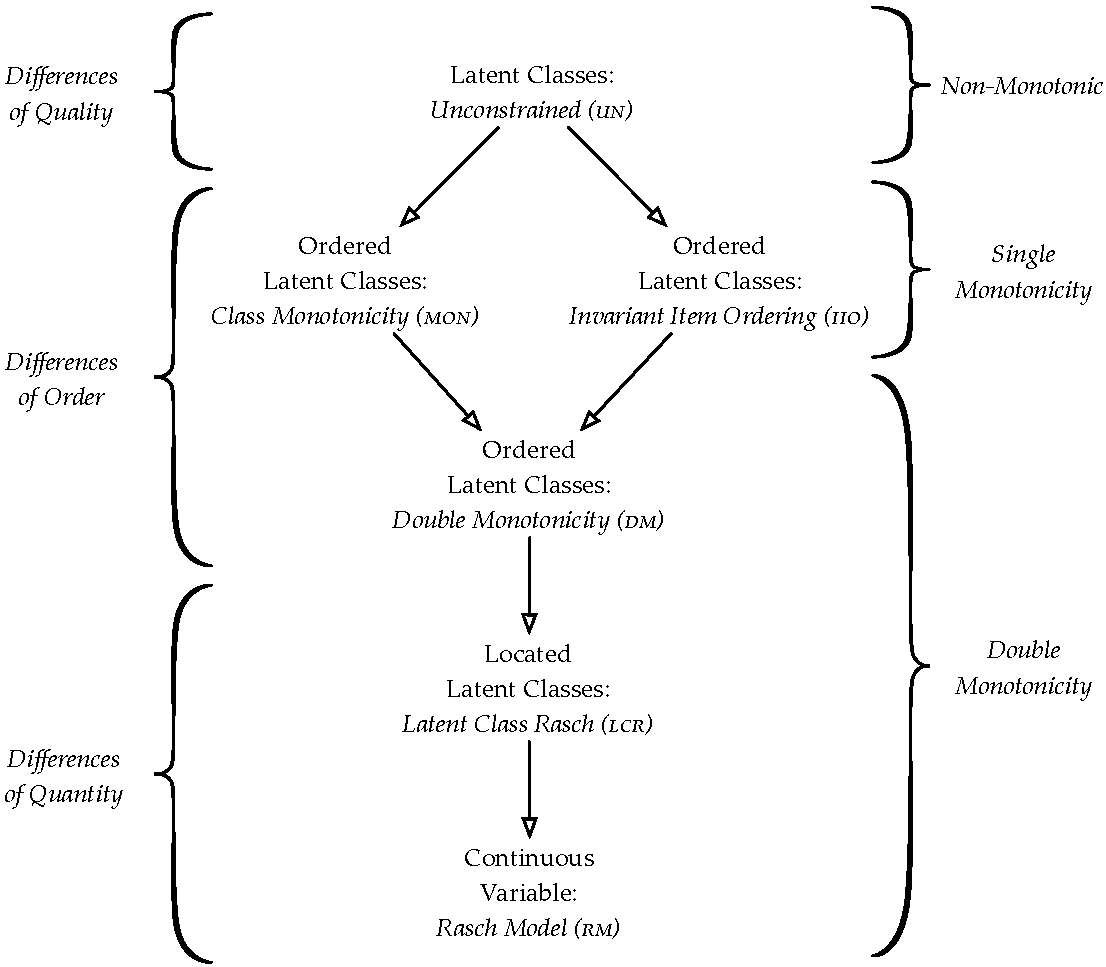
\includegraphics[width=0.75\textwidth]{./figs/Structure3.pdf} \\

}


%models and equations
\frame[allowframebreaks]{

    \frametitle{Six Latent Variable Models}

    \begin{enumerate}
    \parskip 9pt
        \item Unconstrained Latent Class Model (\textsc{un}):
            \begin{equation*} \label{eqn:lcabeta}
                \mathrm{logit} [ Pr(x_{ic} = 1 | c)] = \mathrm{logit} [\pi_{i|c}] = \beta_{ic}
            \end{equation*}

        \item Ordered Latent Class Model with Class Monotonicty (\textsc{mon}):
            \begin{eqnarray*} \label{eqn:monbeta}
               \mathrm{logit} [ Pr(x_{ic} = 1 | c)] = \mathrm{logit} [\pi_{i|c}] = \beta_{ic}, \\
               \beta_{ic} \leq \beta_{ic'} \mbox{ for all $c < c'$ and for all $i$} \nonumber
            \end{eqnarray*}

        \item Ordered Latent Class Model with Invariant Item Ordering (\textsc{iio}):
            \begin{eqnarray*} \label{eqn:iiobeta}
               \mathrm{logit} [ Pr(x_{ic} = 1 | c)] = \mathrm{logit} [\pi_{i|c}] = \beta_{ic}, \\
               \beta_{ic} \leq \beta_{i'c} \mbox{ for all $i < i'$ and for all $c$} \nonumber
            \end{eqnarray*}

        \item Ordered Latent Class Model with Double Monotonicity (\textsc{dm}):
            \begin{eqnarray*} \label{eqn:dmbeta}
               \mathrm{logit} [ Pr(x_{ic} = 1 | c)] = \mathrm{logit} [\pi_{i|c}] = \beta_{ic}, \\
               \beta_{ic} \leq \beta_{ic'} \mbox{ for all $c < c'$ and for all $i$} \nonumber, \\
               \beta_{ic} \leq \beta_{i'c} \mbox{ for all $i < i'$ and for all $c$} \nonumber
            \end{eqnarray*}

        \item Located Latent Class Model or Latent Class Rasch Model (\textsc{lcr}):
            \begin{equation*} \label{eqn:LCR}
                logit [ Pr(x_{ic} = 1 | \theta_c, \delta_i)] = \theta_c - \delta_i
            \end{equation*}

        \item Rasch Model (\textsc{rsh}):
            \begin{equation*}
                \label{eqn:RSH}
                logit [ Pr(x_{ip} = 1 | \theta_p, \delta_i)] = \theta_p - \delta_i
            \end{equation*}
    \end{enumerate}

}


\begin{frame}
    \frametitle{Additive Conjoint Measurement (\textsc{acm})}

    % From Ben's abstract in Psychometrika:

    \begin{itemize}
        \item The axioms of additive conjoint measurement provide a means of testing the hypothesis that testing data can be placed onto a scale with equal-interval properties.
        \begin{itemize}
            \item Solvability, 
            \item the Archimedean Condition and,
            \item Cancellation axioms.
        \end{itemize}
        \item However, the axioms are difficult to verify given that item responses may be subject to measurement error.
    \end{itemize}

\end{frame}

\begin{frame} %bd
    \frametitle{Cancellation axioms}
    Single cancellation: Rows or columns can be consistently ordered.%bd
    %bd [set of matrices used to explain]

    Easiest to see in a $3 \times 3$ matrix formed by the selection of 3 items and 3 abilities:
    \[
    \begin{array}{ccc}
      \cdot&x_{12} &x_{13}  \\
      x_{21}&\cdot&x_{23} \\
      x_{31} & x_{32}&\cdot\\
    \end{array}.
    \]
    Two forms: 
    \begin{enumerate}
    \item If $x_{21}<x_{12} \& x_{32}<x_{23} \text{then} x_{31}<x_{13}$. 
    \item If $x_{21}>x_{12} \& x_{32}>x_{23} \text{then} x_{31}>x_{13}$. 
    \end{enumerate}
    Key is that double cancellation imposes some order on the very messy minor diagonal.

\end{frame}

\begin{frame}
    \frametitle{Applying the axioms of \textsc{acm}}

    \begin{itemize}
        \item Domingue expanded and improved a Bayesian method for imposing order restrictions from additive conjoint measurement while estimating the probability of a correct response.
        \item This method allows the examination of the single and double cancelation axioms by examining the relevant cancellation constraints and estimating credible intervals to check if observed data laid within.
        \item Domingue (In Press) applied the methodology to confirm if the use of the Rasch Model was supported by a reading assessment intentionally designed to support an equal-interval scaling.
    \end{itemize}


\end{frame}

\begin{frame}

    \frametitle{The Framework and the Axioms}

        %temporal until I prepare the new figure
        \centering 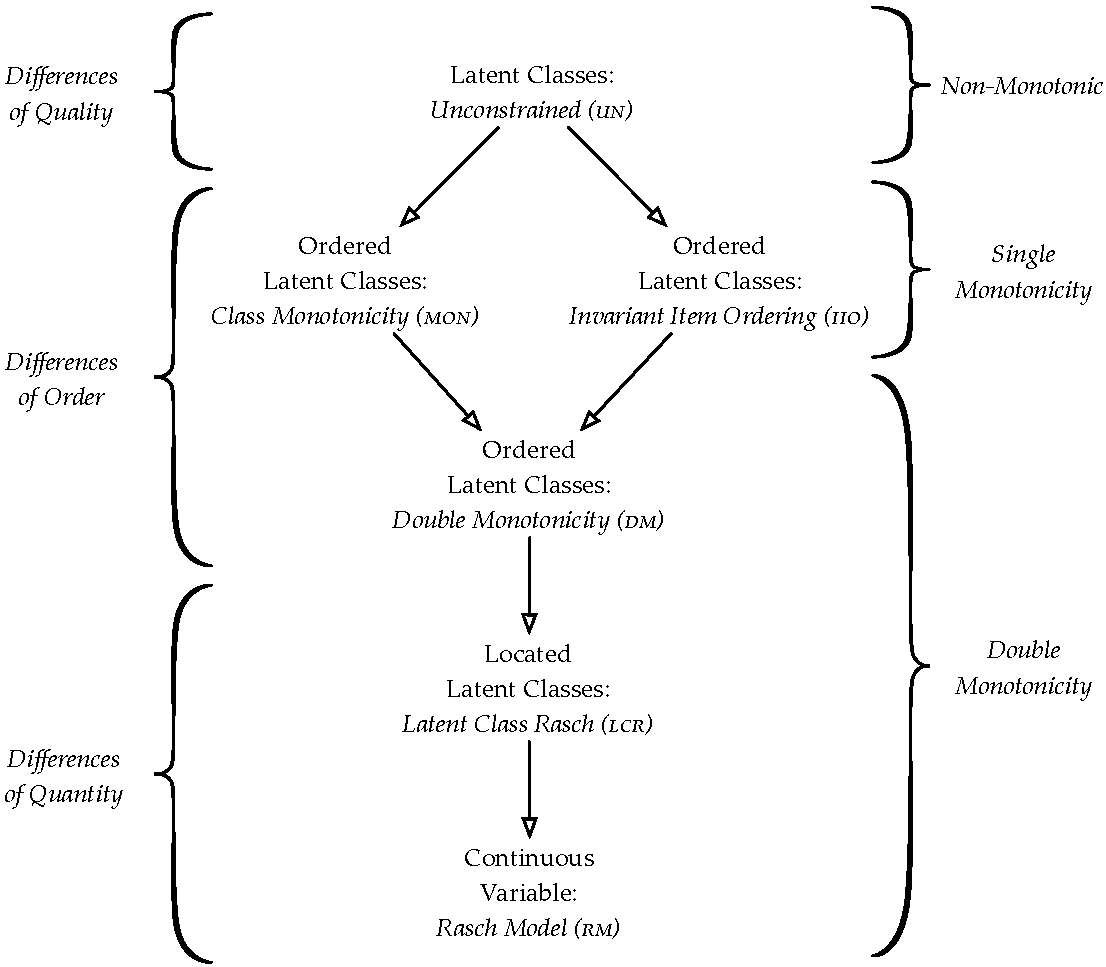
\includegraphics[width=0.75\textwidth]{./figs/Structure3.pdf} \\


\end{frame}


\section{Study design}

\begin{frame}
    \frametitle{Hypotheses/Questions }
    
    \begin{enumerate}
    \item Data generated under an \textsc{un} model should yield the most violations.
    \item The ammount of single cancelation violations under the \textsc{mon} and \textsc{iio} models should be similar.
    \item The \textsc{dm} model should comply with both single cancelations, but not with double cancelation.
    \item The \textsc{lcr} and \textsc{rm} should have the smalles number of violations.
    \item In summ, the expected order is:
        \begin{itemize}
            \item \textsc{un} > ( \textsc{mon} $\sim$ \textsc{iio} ) > \textsc{dm} > ( \textsc{lcr} $\sim$ \textsc{rm} )
        \end{itemize}
    \end{enumerate}
    
    If these hypotheses hold, then we potentially have a fairly straightforward criteria to recover the generating latent structure. 

\end{frame}

\begin{frame}
    \frametitle{Simulation design}

    generate data under each of six models
    
    1000 people in 6 latent classes and 50 items in 6 latent groups
    
    50 replications for each model

\end{frame}

\begin{frame}
    \frametitle{Analysis}

    ConjointChecks, each single cancellation and double cancellation
    
    \% weighted violations

\end{frame}


\section{Results}

\begin{frame}
    \frametitle{Double cancellation}

    [include figure]

\end{frame}

\begin{frame}
    \frametitle{Single cancellation -- Person ordering}

    \centering 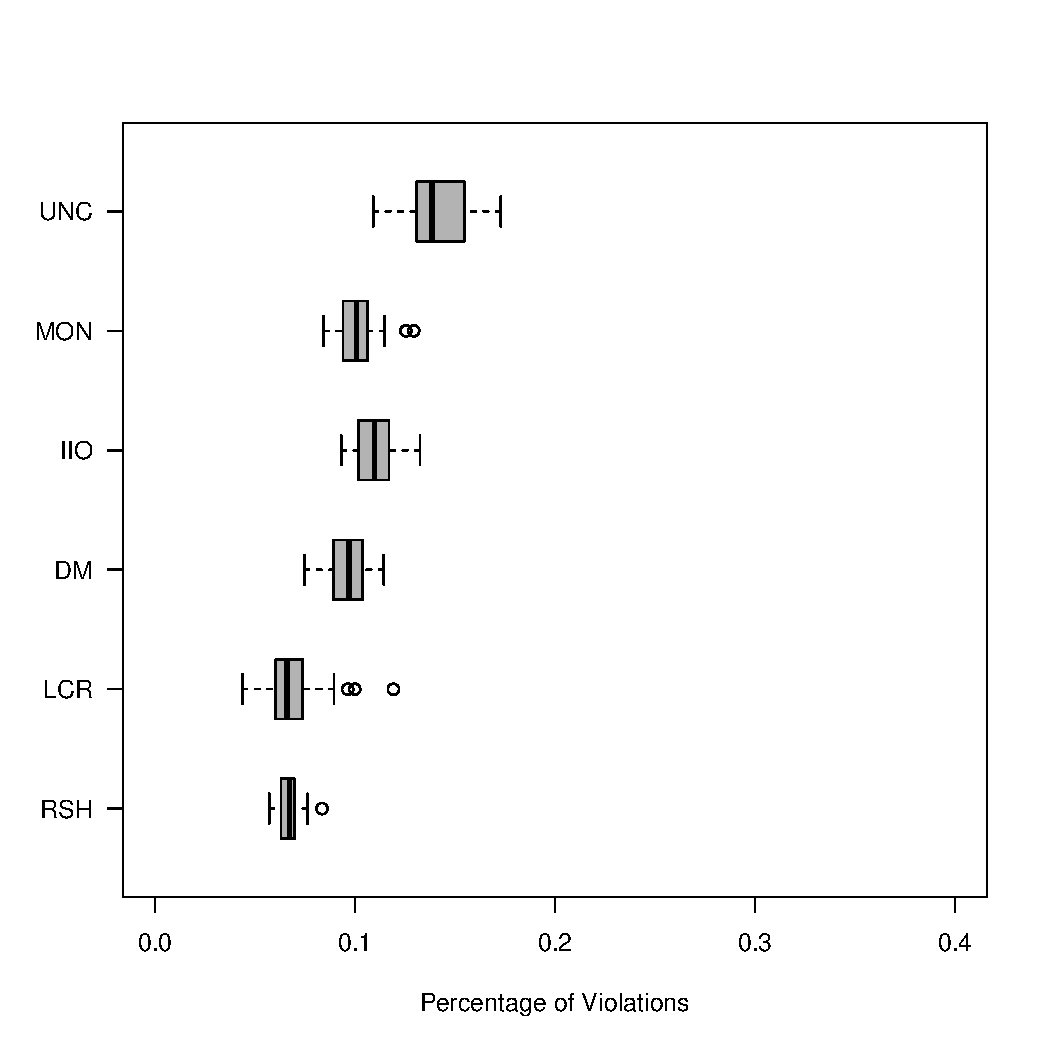
\includegraphics[width=0.75\textwidth]{./figs/violations_columns_weighted.pdf}

\end{frame}

\begin{frame}
    \frametitle{Single cancellation -- Item ordering}

    \centering 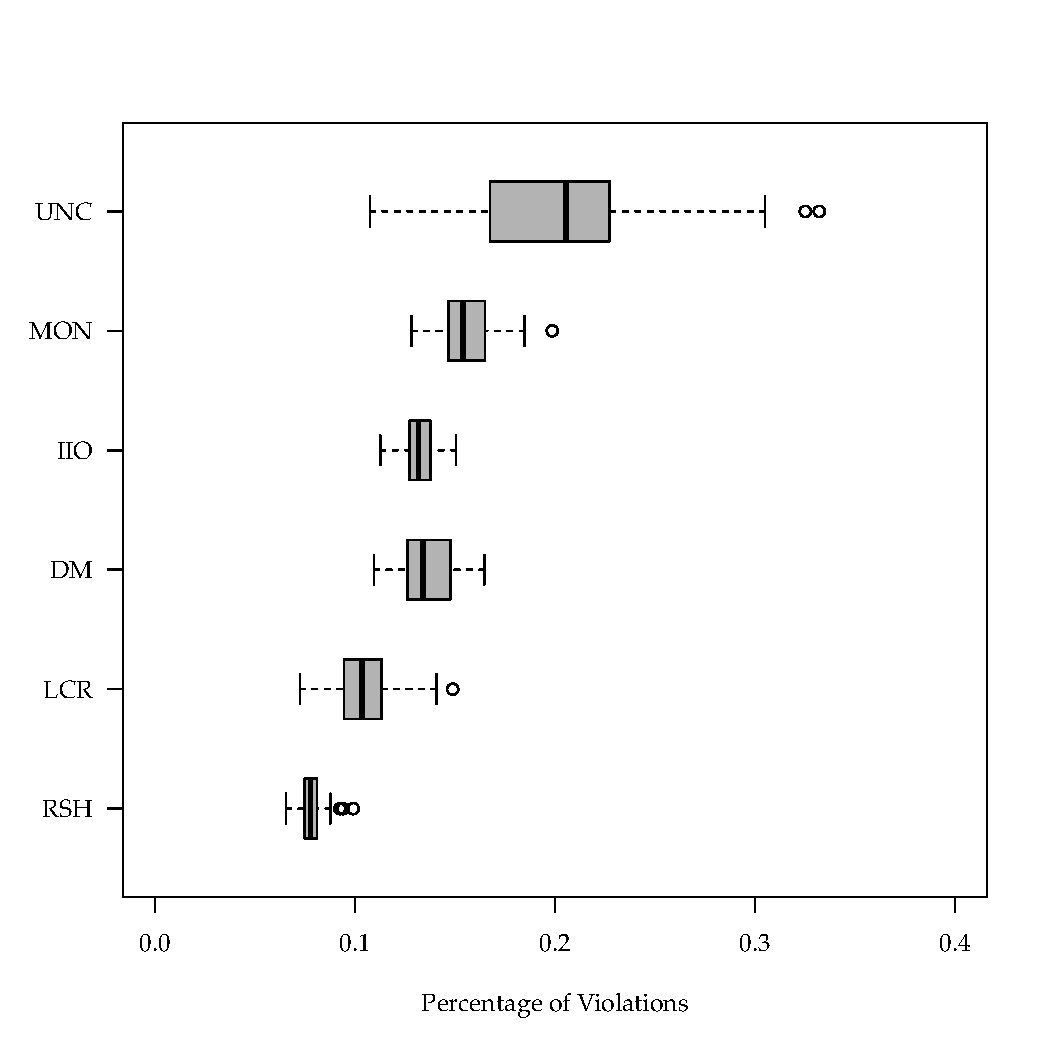
\includegraphics[width=0.75\textwidth]{./figs/violations_rows_weighted.pdf}

\end{frame}


\section{Discussion}

\begin{frame}
    \frametitle{Person monotonicity versus item ordering}

    precision / aggregation
    
    how this simulation is different from how we usually treat persons and items

\end{frame}

\begin{frame}
    \frametitle{Reconsidering double cancellation}

\end{frame}

\begin{frame}
    \frametitle{Further thoughts}

\end{frame}

\frame[contactinfo]{

    \begin{center}

    \Large Applying the Axioms of Additive Conjoint Measurement to a Hierarchy of Latent Variable Models

    \vspace{10mm}

    \small

    \begin{tabular}{rl}

        xxx@xxx.xxx          & \textsc{Benjamin Domingue} \\
        dti@berkeley.edu     & \textsc{David Torres Irribarra} \\
        rdiakow@berkeley.edu & \textsc{Ronli Diakow}
        
    \end{tabular}
    
    \end{center}

    \vspace{10mm}

%    \scriptsize
%    \hspace{5mm} Torres Irribarra, D., and Diakow, R.  (2011, July).  Model Selection for Tenable Assessment: Selecting a Latent Variable Model by Testing the Assumed Latent Structure.  Paper presented at the 76th Annual and 17th International Meeting of the Psychometric Society, Hong Kong.


}


%back-up slides
\appendix

%fix so slide numbering ignores back-up slides
\newcounter{finalpage}
\setcounter{finalpage}{\value{page}}
\newcounter{finalframe}
\setcounter{finalframe}{\value{framenumber}}
\setbeamertemplate{footline}{}

\begin{frame}

    \centering Appendix Slides

\end{frame}

%fix so slide numbering ignores back-ups
\setcounter{page}{\value{finalpage}}
\setcounter{framenumber}{\value{finalframe}}

\end{document}


\begin{frame}
    \frametitle{}

\end{frame}